\section{Encountered difficulties}
Debugging is a rare skill, only few resources are available. We can point out some difficulties that we have seen during internship :

\subsection{Hardware issues}
Hardware problems were a real bottlenecks, as they are more difficult to locate and troubleshoot.
\subsubsection{JTAG tampering}
Some manufacturers try to hide \textbf{JTAG connectors} to make it difficult to access (\textit{due to security reasons}). Beaglebone black wireless is an example of those boards. Soldering a JTAG connector was mandatory (\textit{it is not easy on those tiny devices}).

\textbf{\color{orange}Note : } sometimes JTAG connection is encrypted or even damaged by manufacturers (\textit{but this is rare}). 
More can be said about \textbf{JTAG} as connectors are different and pinout definition is not always easy to find (solutions like \textbf{JTAGulator} at : {\color{blue}\url{https://hackaday.com/2013/10/02/jtagulator-finds-debug-interfaces/}} may be helpful).
\subsubsection{OpenOCD hardware interfacing}
As mentionned previously, \textbf{OpenOCD} is a hardware debugging solution (it is complicated). It took me 1.5 week to understand how to make a correct hardware setup (\textbf{Figure \ref{OpenOCD ACK error due to incorrect TDI connection}}).


\begin{figure}[H]
		\centering
        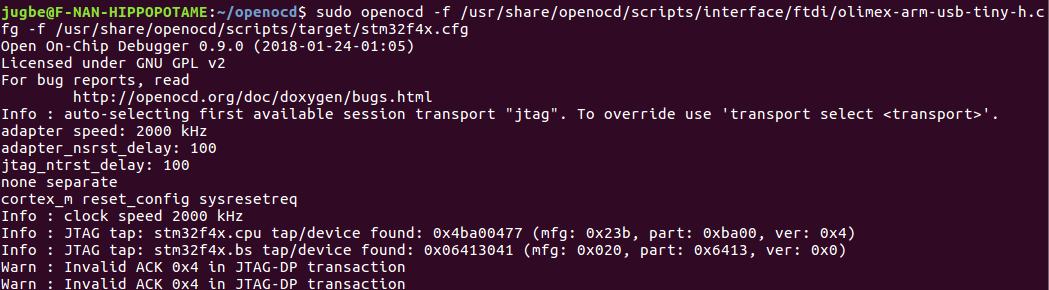
\includegraphics[scale=0.40]{img/issues/tdi-not-connected-openocd.png}
        \caption{OpenOCD ACK error due to incorrect TDI connection}
        \label{OpenOCD ACK error due to incorrect TDI connection}
    \end{figure}


\subsubsection{OpenOCD's compliant adapter}
Adapters are expensive, adapters that are compatible with OpenOCD are difficult to find.\\
\textbf{Solution : } We used ARM-USB-TINY-H ({\color{blue} \url{https://www.olimex.com/Products/ARM/JTAG/ARM-USB-TINY-H/}}) from Olimex.

\subsection{Software}

\subsubsection{Debugging symbols}
Most kernels in production are compiled removing this option. The advantage is to reduce kernel's image size, however, tools like : GDB becomes practically useless as they require debugging symbols (see \textbf{Figure \ref{GDB is practically useless without debugging symbols}}). 

\begin{figure}[H]
		\centering
        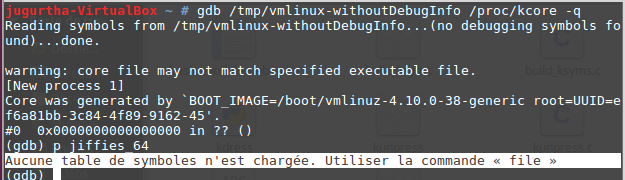
\includegraphics[scale=0.40]{img/issues/no-debug-symbol.png}
        \caption{GDB is practically useless without debugging symbols}
        \label{GDB is practically useless without debugging symbols}
    \end{figure}


Some solutions exist to reconstruct it (without recompiling the kernel) and works only fine on x86 (see {\color{blue}\url{https://github.com/elfmaster/kdress}}).




Even worse, /proc/kcore does not exist on most embedded systems (like ARM)\footnote{More details about /proc/kcore are available at :  {\color{blue}\url{https://lwn.net/Articles/45315/}}}.


\subsubsection{Yama blocks ptrace}
Yama is a security module that disables ptrace. GDB, strace and ltrace make use of ptrace which must be enabled.\\

\textbf{\color{orange}Solution : } enable ptrace as shown in {\color{red}subsection {\color{blue}\ref{System calls and library calls}}}
\subsubsection{JTAG lockers}
Even if OpenOCD's hardware interfacing is correct, some boards have software protections to disable JTAG. Raspberry PI is an example. The firmware blocks any JTAG connection by default. Workarounds were made to disable such mechanisms.\\

\textbf{\color{orange}Solution : } enable JTAG as shown in {\color{red}subsection {\color{blue}\ref{Linux hardware debugging with OpenOCD}}}
\subsubsection{Disabled serial communication}
Serial communication can be disabled on some devices, \textbf{Raspberry PI} is an example of those. It took me 3 hours to figure out the reason of unsuccessful connection (\textit{even if hardware setup is correct} as shown in \textbf{Figure \ref{Hardware setup for serial communication - Raspberry PI 3}}). 


\begin{figure}[H]
		\centering
        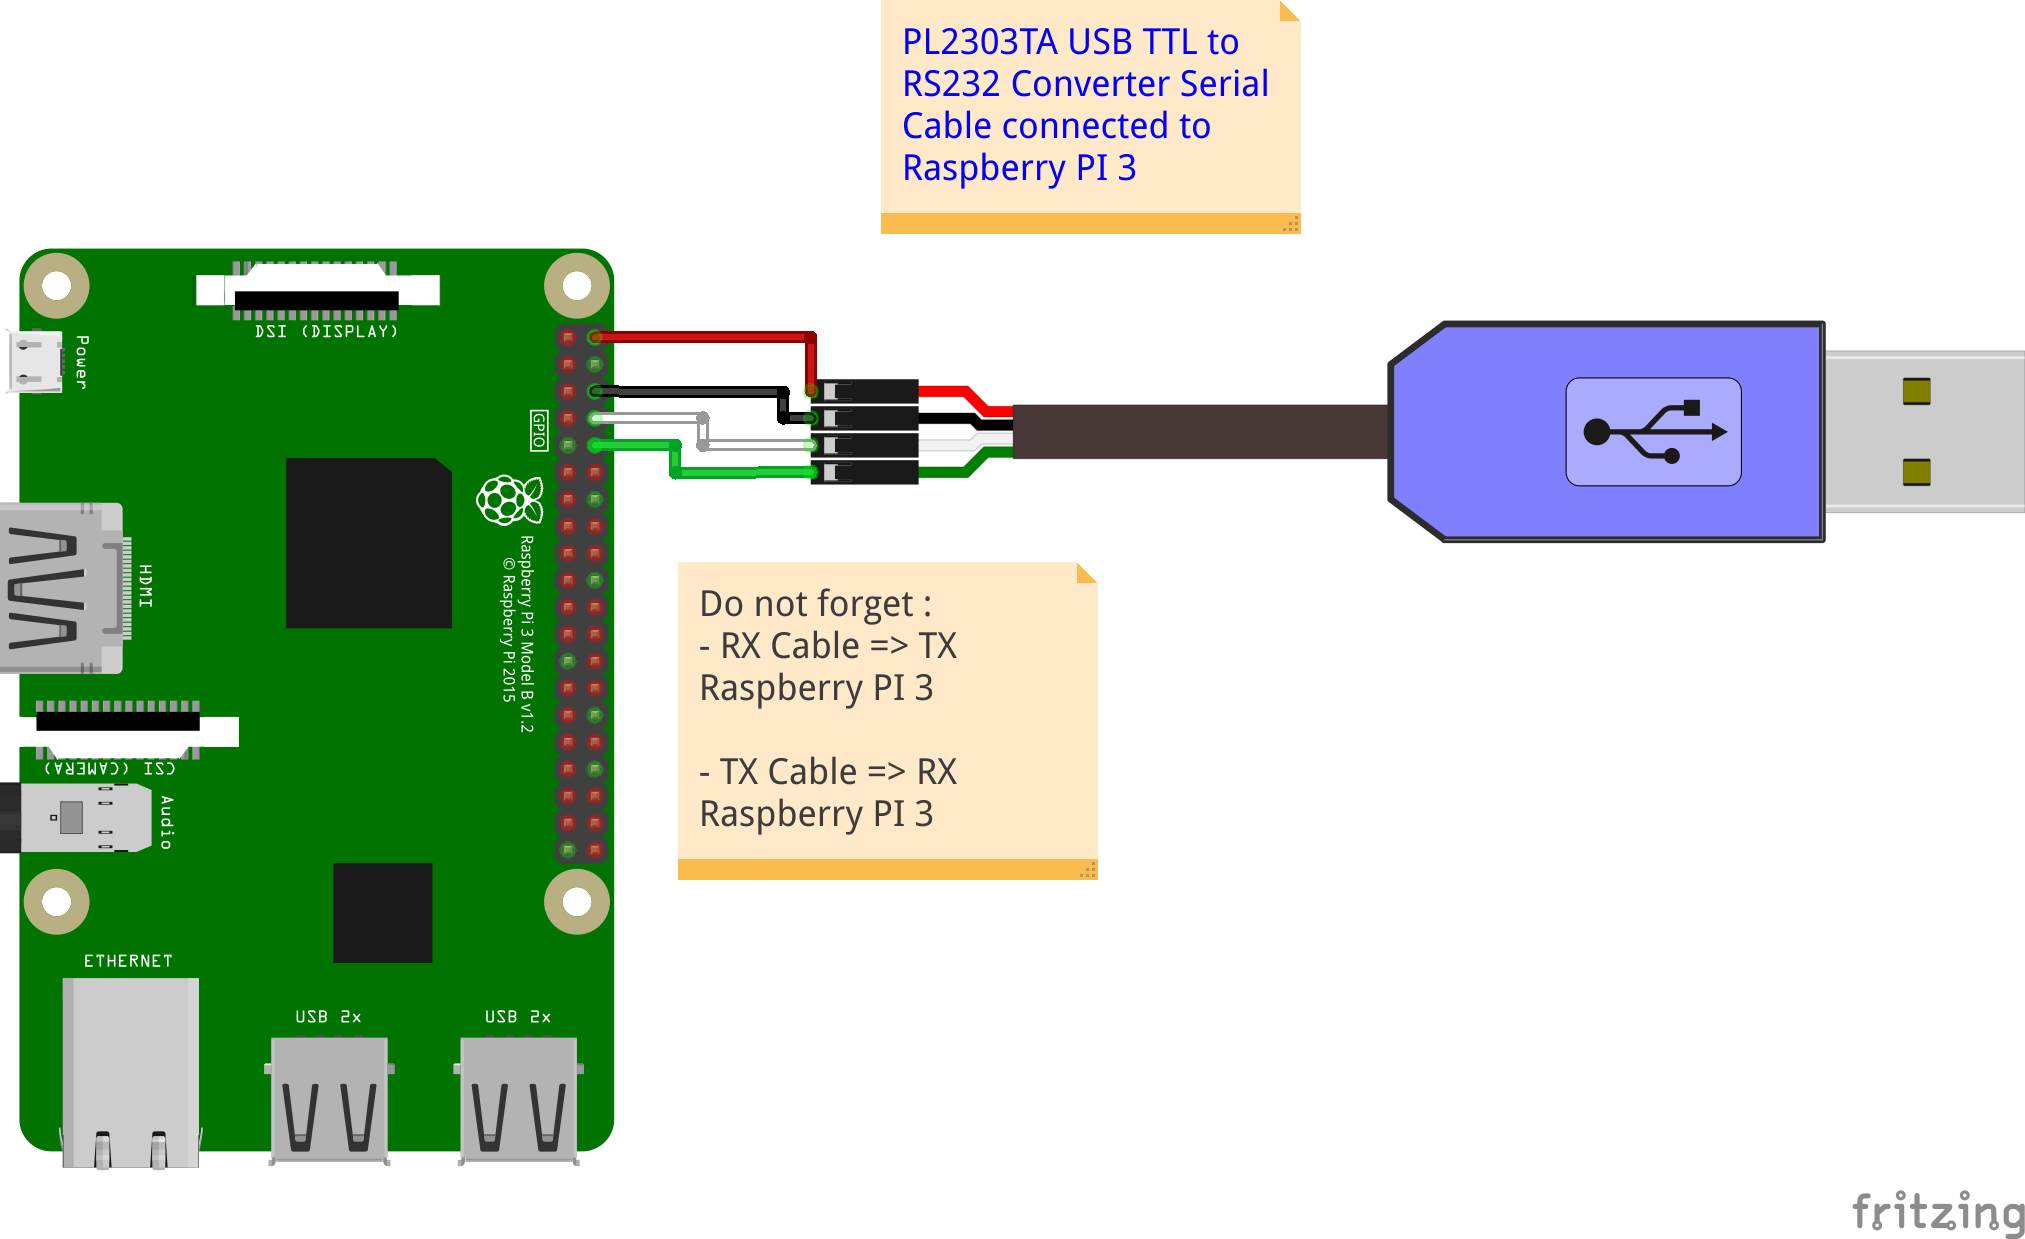
\includegraphics[scale=0.40]{img/issues/USB-Serial-cable-To-Raspberry-PI-3_bb.png}
        \caption{Hardware setup for serial communication - Raspberry PI 3}
        \label{Hardware setup for serial communication - Raspberry PI 3}
    \end{figure}



\textbf{\color{orange}Solution : } To enable serial communication on Raspberry PI, follow the steps presented at : {\color{blue}\url{https://hallard.me/enable-serial-port-on-raspberry-pi/}}.
\subsubsection{OpenOCD scripts}
As We have already mentionned, OpenOCD does not support every board. Custom configuration files must be written to include new platforms. We have made scripts generation easier with OESdebug, provided step by step documentation of OpenOCD and an animation that helps to understand more ({\color{blue} \url{https://jugurthab.github.io/debug_linux_kernel/zero-to-hero-openocd.html}}).\\

{\color{orange}Solution : } see {\color{red}subsection {\color{blue}\ref{Linux hardware debugging with OpenOCD}}} (go to \og \textit{OpenOCD made easy with OESdebug} \fg).


\subsubsection{DebugFs absent}
Security engineers drop down \textbf{DebugFs} support as it allows anyone to get insight into the Kernel. Only Hardware debugging can help in such case.\\
We point the fact that tracers will be difficult to port and used as some rely heavily on \textbf{DebugFS}.
